\documentclass{beamer}
\usepackage{graphicx}
\usepackage{listings}
\usepackage{hyperref}
\usepackage{tikz}
\usetheme{Antidot}
\begin{document}
\title{Maintaining a World of Warcraft addon}
\author{Pierre Sassoulas}
\date{2020-07-01}


\newcommand{\shrug}[1][]{%
\begin{tikzpicture}[baseline,x=0.8\ht\strutbox,y=0.8\ht\strutbox,line width=0.125ex,#1]
\def\arm{(-2.5,0.95) to (-2,0.95) (-1.9,1) to (-1.5,0) (-1.35,0) to (-0.8,0)};
\draw \arm;
\draw[xscale=-1] \arm;
\def\headpart{(0.6,0) arc[start angle=-40, end angle=40,x radius=0.6,y radius=0.8]};
\draw \headpart;
\draw[xscale=-1] \headpart;
\def\eye{(-0.075,0.15) .. controls (0.02,0) .. (0.075,-0.15)};
\draw[shift={(-0.3,0.8)}] \eye;
\draw[shift={(0,0.85)}] \eye;
% draw mouth
\draw (-0.1,0.2) to [out=15,in=-100] (0.4,0.95);
\end{tikzpicture}}

\frame{\titlepage}

\AtBeginSection[]
{
    \begin{frame}
        \frametitle{Table of Contents}
        \tableofcontents[currentsection]
    \end{frame}
}

\section{Introduction}

\subsection{Definition}

\frame{\frametitle{Definition}
    \begin{columns}
        \begin{column}{0.6\textwidth}
            \begin{block}{What is World of Warcraft (WOW)}
                \begin{itemize}
                    \item Massively multiplayer online role-playing game (MMORPG)
                    \item So successful that all competitors were deemed unsuccessful to this day
                    \item 7 expansions updated and delivered continuously since 2004
                \end{itemize}
            \end{block}
        \end{column}
        \begin{column}{0.4\textwidth}
            \begin{center}
                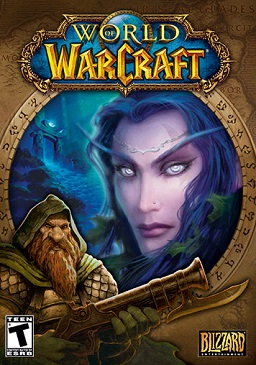
\includegraphics[width=0.8\textwidth]{WoW_Box_Art1.jpg}
                \source{WOW Official Website}
             \end{center}
        \end{column}
    \end{columns}
}

\frame{\frametitle{Definition}

    \begin{block}{WOW classic VS WOW retail ?}
        \begin{itemize}
            \item WOW classic : Original WOW without expansion
            \item WOW retail : Current updated WOW with 7 added expansions
        \end{itemize}
    \end{block}

    \begin{block}{What is an addon ?}
        An AddOn is some files that you can put in your game folder that improve your interaction with the game
        (i.e. make it easier to play, or give you more information about what's going on in the game).
        \source{https://wowwiki.fandom.com/wiki/AddOn}
    \end{block}

    \begin{block}{What is Lua?}
        Programming language used for developping addons in WOW.
    \end{block}

}

\subsection{Context}

\frame{\frametitle{The context}
    \begin{block}{The great WOW classic hype of summer 2019}
        \begin{itemize}
            \item 13 August 2019 : European beta for WOW classic
            \item 27 August 2019 : Official launch of WOW classic
        \end{itemize}
    \end{block}

    \begin{center}
        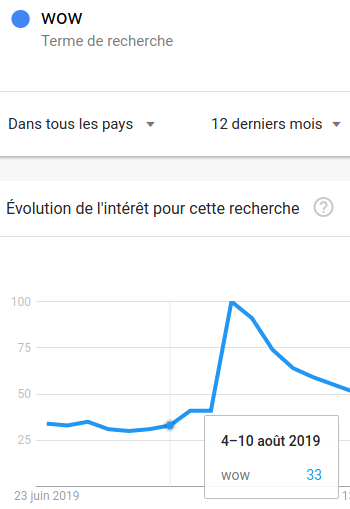
\includegraphics[width=0.3\textwidth]{wow_summer_hype.png}
        \source{Google trends}
    \end{center}
}

\frame{\frametitle{The context : WOW Classic}

    \begin{block}{Low level in beta realisation : In WOW classic optimizing bag is critical again !}
        \begin{itemize}
            \item No knowledge of item's prices until you sell them,
            \item No knowledge of item's stack size until it overflow
            \item Sparse bag slots, and numerous items
            \item Never enough money to buy basic necessities
        \end{itemize}
    \end{block}

    \begin{center}
        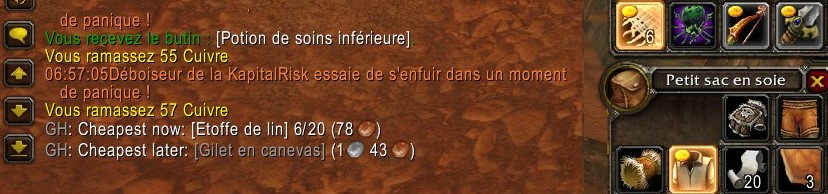
\includegraphics[width=0.8\textwidth]{../examples/red_glow.jpg}
        \source{Bouzrogue, addon developer}
    \end{center}
}

\frame{\frametitle{The context : WOW Classic}

    \begin{block}{The 14th of August I had}
        \begin{itemize}
            \item A burning desire to play WOW classic, and an idea for a classic addon, following 5h of beta
            \item No prior Lua or WOW addon development experience
            \item Only WOW retail available for testing until the 27th
        \end{itemize}
    \end{block}
    \begin{center}
        
\includegraphics[width=0.3\textwidth]{better_than_regular_programming.png}
        \source{South Park, Make love not Warcraft}
    \end{center}
}


\subsection{The idea}

\frame{\frametitle{The idea}
    \begin{block}{Make bag management less time-consuming and memory intensive}
        \begin{itemize}
            \item Gives indication about prices and stacks outside of vendor
            \item Optimize throwing vendor-only objects
            \item Optimize bag spaces within a dungeon group
            \item Nice user-friendly print telling you what to do
            \item No bag addon integration
        \end{itemize}
    \end{block}
    \begin{center}
        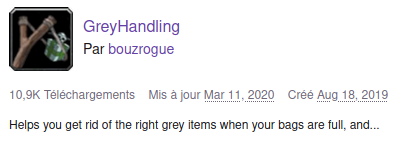
\includegraphics[width=0.6\textwidth]{5daystoprod.png}
        \source{Curseforge}
    \end{center}
}

\frame{\frametitle{Feature request starts flowing in}

    \begin{block}{Friend and guildies required features}
        \begin{itemize}
            \item How can a print be "nice" ?
            \item Integrate with ALL their addons for bags
            \item Give visual cue in item tooltip
        \end{itemize}
    \end{block}

    \begin{center}
        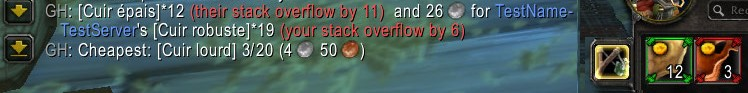
\includegraphics[width=0.8\textwidth]{../examples/bagnon_integration.jpg}
        \source{Bouzrogue, addon developer}
    \end{center}
}

\frame{\frametitle{Demonstration}
\begin{block}{Basic use during solo play}
    \begin{center}
        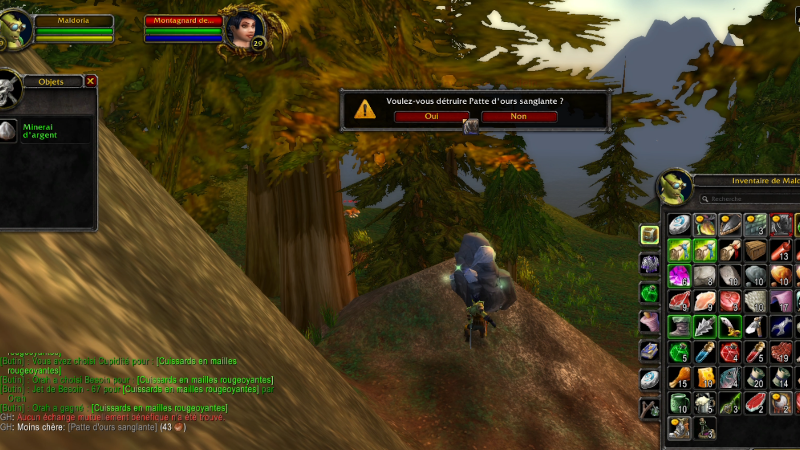
\includegraphics[width=0.7\textwidth]{miniature_basic_example.png}
        ~~ \\
        \href{https://youtu.be/eOInQ0ww6Qk}{Click this text to view demo}
        \source{Youtube, https://youtu.be/eOInQ0ww6Qk}
    \end{center}
\end{block}
}

\frame{\frametitle{Demonstration}
\begin{block}{Item exchange during dungeon based on analysis of group events}
    \begin{center}
        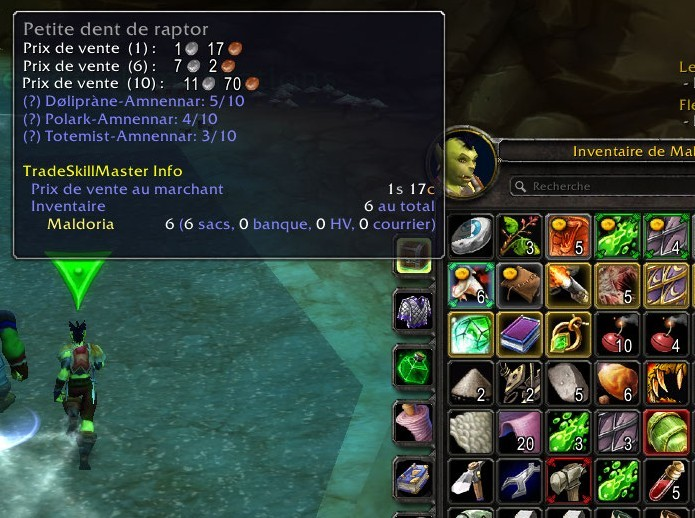
\includegraphics[width=0.46\textwidth]{combductor_integration.jpg}
        \source{Bouzrogue, addon developer}
    \end{center}
\begin{itemize}
    \item GreyHandling found beneficial exchanges (green items)
    \item Or you can always throw your blacksmith hammer
\end{itemize}


\end{block}
}

\frame{\frametitle{Demonstration}
\begin{block}{Item exchange during dungeon based on analysis of group events}
    \begin{center}
        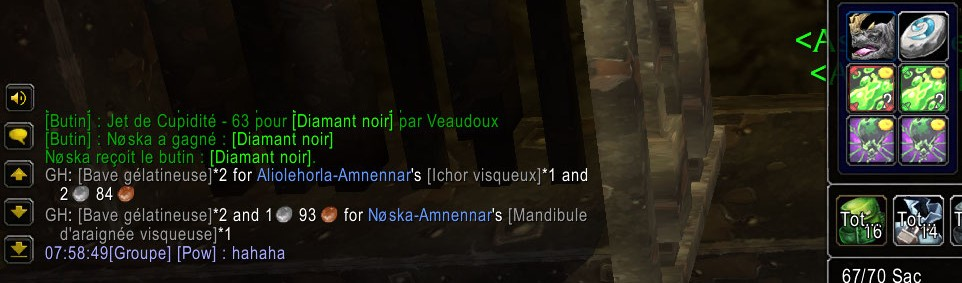
\includegraphics[width=0.7\textwidth]{team_exchange.jpg}
        \source{Bouzrogue, addon developer}
    \end{center}
\end{block}
\begin{block}{Problem with this approach}
    \begin{itemize}
        \item It's complicated to ask for something in return
        \item Giving away to teammates is faster (Hopefully its good for your reputation on the server)
    \end{itemize}
\end{block}
}

\frame{\frametitle{Demonstration}
    \begin{block}{Direct communication between GreyHandling instances}
        \begin{center}
            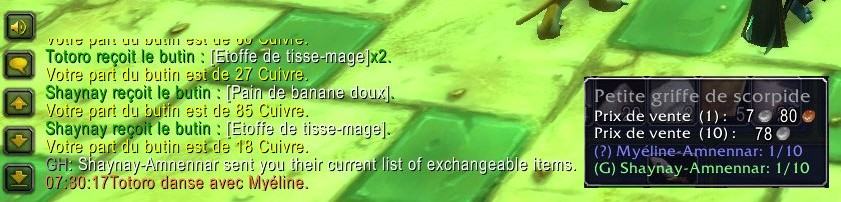
\includegraphics[width=0.9\textwidth]{itemtooltip1.jpg}
            \source{Bouzrogue, addon developer}
        \end{center}
    \end{block}
    \begin{block}{No video demonstration}
        \begin{itemize}
            \item My friends were bored with the game really fast \shrug\
            \item Also, surprisingly, not everyone use GreyHandling yet
        \end{itemize}
    \end{block}
}



\section{Development environment}

\subsection{IDE setup with Pycharm}

\frame{\frametitle{Plugin for Pycharm}

    \begin{block}{Lua}
        \begin{itemize}
            \item Some Automatic FrameXML Injections specific to WOW
            \item At first I chose it because of this, it was a mistake, I very rarely used FrameXML
        \end{itemize}
    \end{block}

    \begin{block}{EmmyLua}
        \begin{itemize}
            \item Auto-completion after parsing your code
            \item And of all of the addons in Interface/Addons (!) (If the Pycharm project is Interface/Addons)
            \item Auto-completion of other addons is an absolute must have
        \end{itemize}
    \end{block}
}

\frame{\frametitle{Development set up}
    \begin{block}{IDE/WOW set up}
        \begin{itemize}
            \item Put your source directory in "Addons/Interface", rename it so it match your .toc
            \item Create a $/reload$ WOW macro so you can apply changes fast
            \item Find a way to launch unit tests
        \end{itemize}
    \end{block}

    \begin{center}
        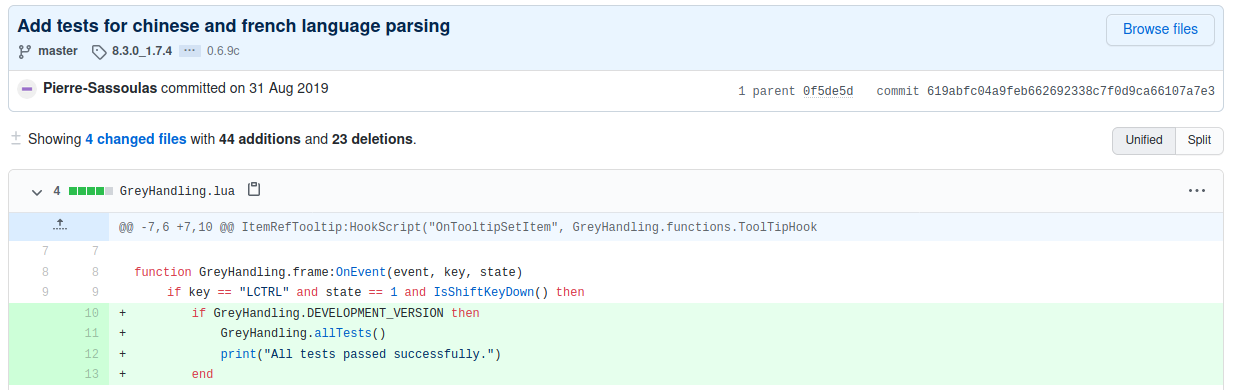
\includegraphics[width=0.9\textwidth]{debug.png}
        \source{github.com GreyHandling 619abfc04a9feb662692338c7f0d9ca66107a7e3}
    \end{center}

}

\subsection{The Lua language}

\frame{\frametitle{Surprising feature n°1}
    \begin{block}{Variables are global by default : Can you guess what's wrong in this commit ?}
        \begin{center}
            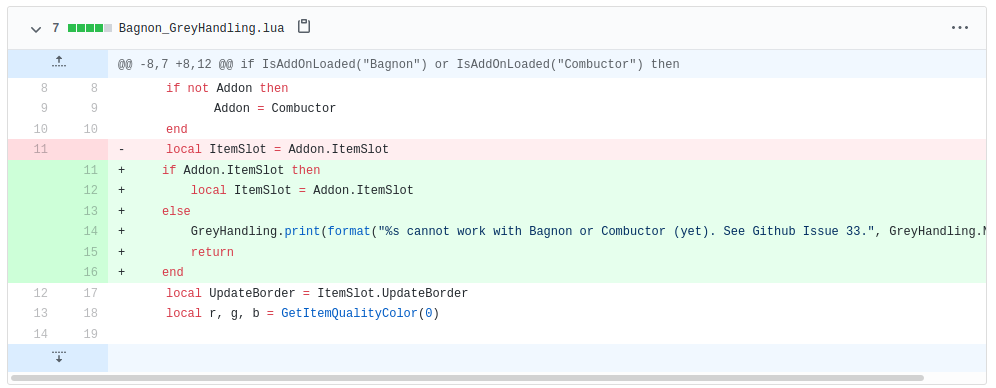
\includegraphics[width=0.8\textwidth]{whats_wrong_with_this.png}
            \source{github.com GreyHandling 4abf6fc89920e438a1a05cf44c6cc8011c8e3949}
        \end{center}
        Yeah, it happened more than one time to me.
    \end{block}
}

\subsection{Tips for begginner}

\frame{\frametitle{Builtin functions are also (horrifyingly) public}

\begin{flushright}
    \begin{quote}
    The WOW API makes blowing the whole leg of other people off really easy.
    \end{quote}
    \small (Almost) Bjarne Stroustrup \normalsize
\end{flushright}
\begin{block}{Don't do that, ever}
   \begin{center}
        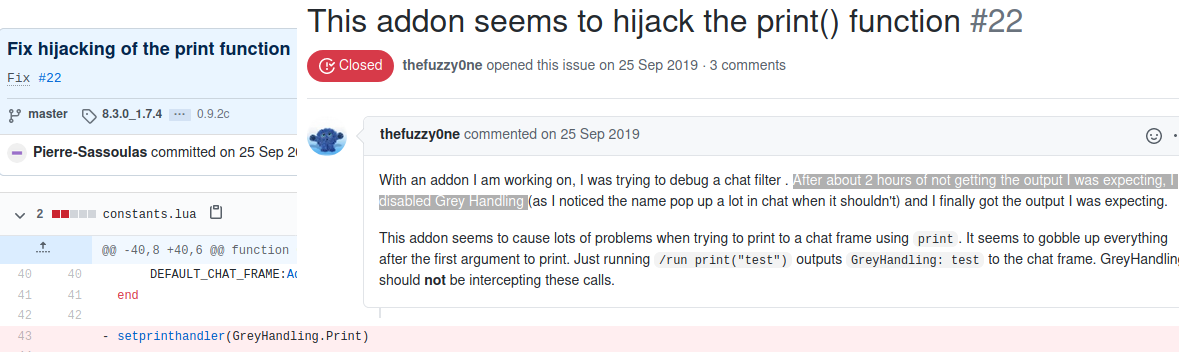
\includegraphics[width=1\textwidth]{hijack_print.png}
        \source{github.com GreyHandling 07ed9c758ea1b4a81092313511359c3c44c757da}
    \end{center}
\end{block}

}

\begin{frame}[fragile]
    \frametitle{Read your failing code's stacktrace}
    \begin{block}{Showing Lua errors in interface:}
        \begin{lstlisting}[label={lst:lstlisting}]
            /console scriptErrors 1
        \end{lstlisting}
        Or if you'd rather click: https://youtu.be/vPVU0zwQJ5o
    \end{block}
    \begin{center}
        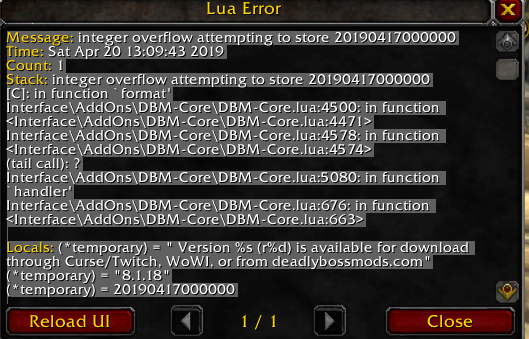
\includegraphics[width=0.4\textwidth]{th1r1sv08ht21.png}
        \source{reddit.com /r/wow/comments/bfgjh0/lua\_errors\_help/}
    \end{center}
\end{frame}

\frame{\frametitle{Evenemential programmation}

    \begin{block}{There is an event mindset to have}
        \begin{itemize}
            \item Don't launch all your code like a script with a keybind
            \item Listen to events and do something only when they happens
            \item Do very specific things for each events
        \end{itemize}
    \end{block}

    \begin{block}{Example : Not doing everything after a keybind...}
        \begin{itemize}
            \item Update the cheapest object after the "UNIT\_INVENTORY\_CHANGED" event
            \item Update item tooltip after the "BAG\_UPDATE\_REQUIRED" event
            \item ...
        \end{itemize}
    \end{block}
}

\frame{\frametitle{Knows your event}

    \begin{block}{Use /etrace}
        \begin{itemize}
            \item Use it in deserted areas to avoid noise
            \item Track events and their arguments
            \item Avoid reading the documentation
            \item If you want to be efficient use the right one
        \end{itemize}
    \end{block}

    \begin{center}
        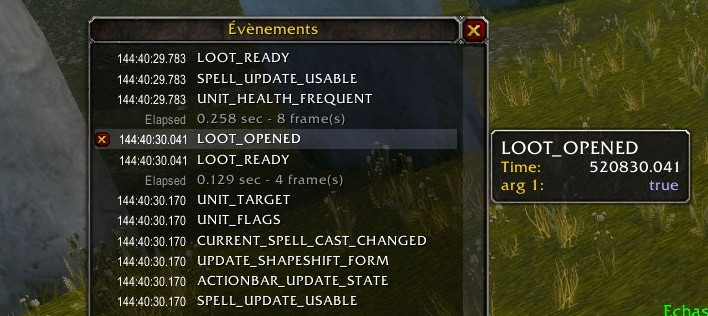
\includegraphics[width=0.48\textwidth]{etrace.jpg}
        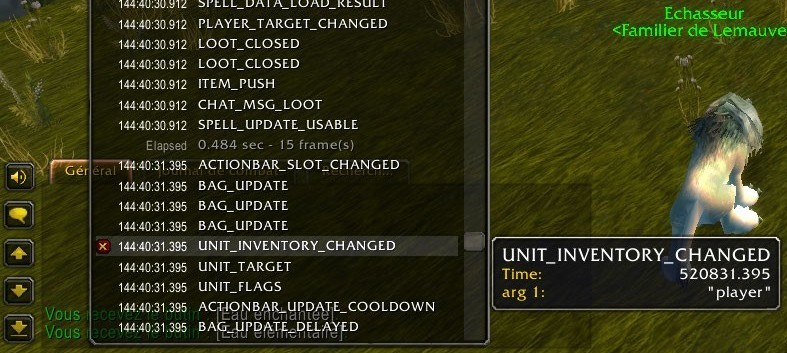
\includegraphics[width=0.48\textwidth]{etrace2.jpg}
        \source{Bouzrogue, addon developer}
    \end{center}

    Not using this from the start made my addon less efficient to this day
    (refactoring would take days).

}

\frame{\frametitle{Resources}

    There is no official resources. Blizzard's internal addon code disapeared some time ago.

    \begin{block}{Useful resources by the community}
        \begin{itemize}
            \item Open-source addons done by cleverer and more knowledgeable WOW developers than you
            \item wowwiki.fandom.com (events, API, XML, and a lot more)
            \item Projects that emulate WOW's API (Ellypse's "wow-ui-source" on github.com for example) for auto-completion
        \end{itemize}
    \end{block}
}



\frame{\frametitle{Expanding functionality and creating new files}
    \begin{block}{Regarding file with a lot of codes inside it}
        \begin{itemize}
            \item Do not create new files when developing
            \item You would need to relaunch WOW for the new file to be taken into account
            \item But do pay that technical debt later !
        \end{itemize}
    \end{block}

    \begin{center}
        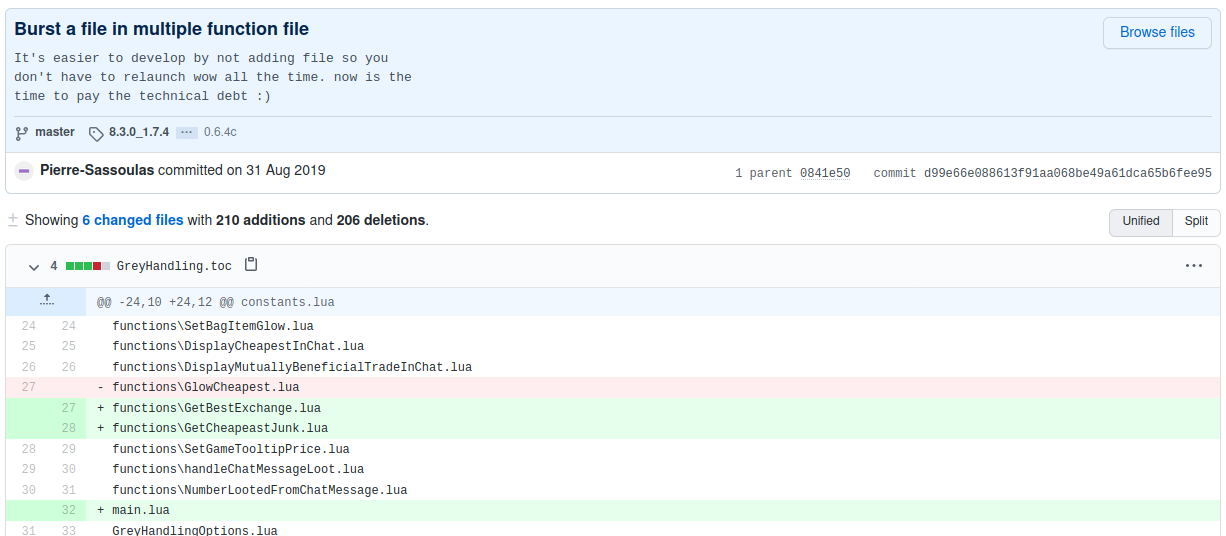
\includegraphics[width=0.8\textwidth]{burst_files.png}
        \source{github.com GreyHandling d99e66e088613f91aa068be49a61dca65b6fee95}
    \end{center}
}

\subsection{Things you may have to deal with}

\frame{\frametitle{Keybinds}

    \begin{block}{Make your keyboard shortcut official}
        \begin{itemize}
            \item It's not that hard, it's a small XML file
            \item If your keybind conflict with user's keybinds, and they can't change yours, they go "bye bye"
        \end{itemize}
    \end{block}
    \begin{center}
        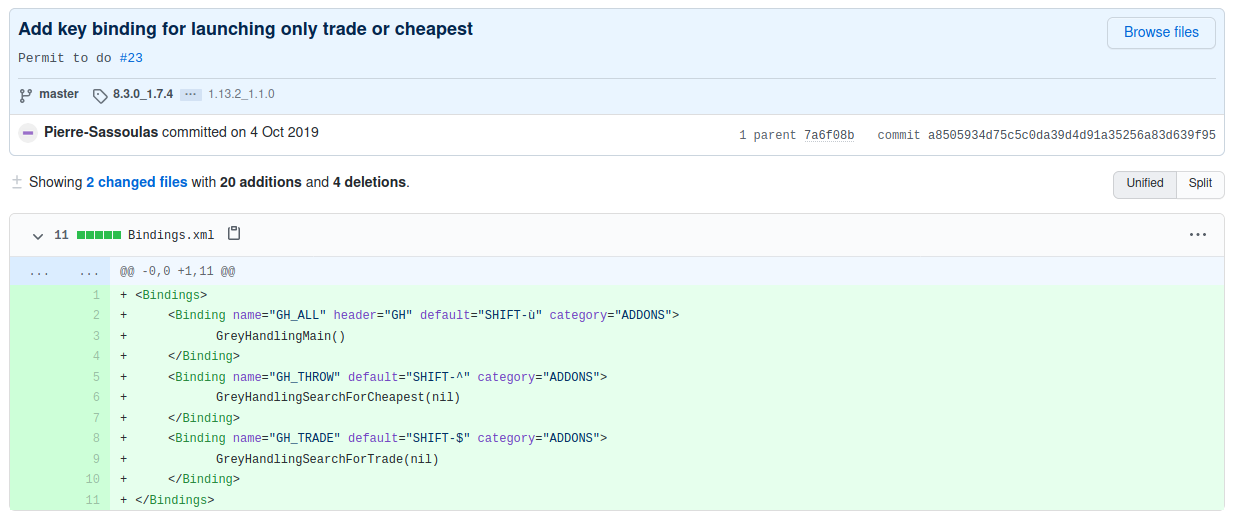
\includegraphics[width=0.8\textwidth]{keybinds.png}
        \source{github.com GreyHandling a8505934d75c5c0da39d4d91a35256a83d639f95}
    \end{center}
}

\frame{\frametitle{Keybinds}
    \begin{center}
        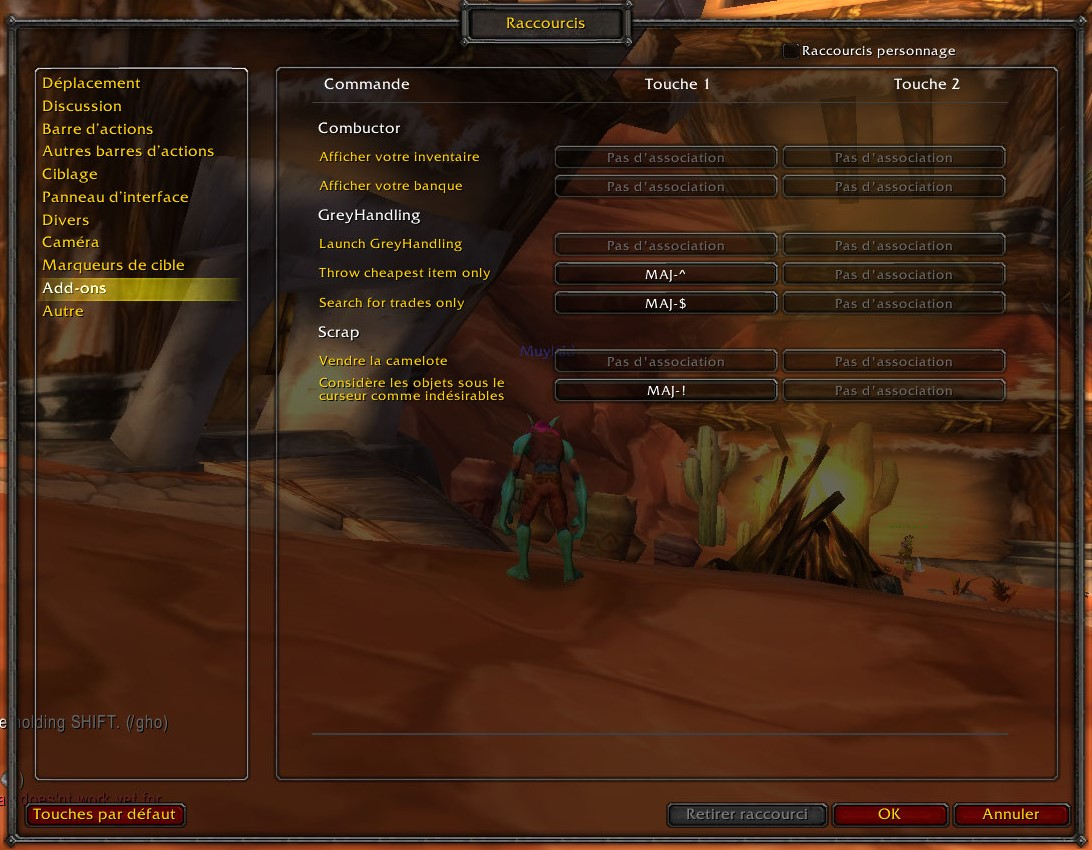
\includegraphics[width=0.7\textwidth]{../examples/keybinding.jpg}
        \source{Bouzrogue, addon developer}
    \end{center}
}

\frame{\frametitle{Option panel}
    \begin{block}{The major pain point during development for me}
        \begin{itemize}
            \item Unless your addon is really simple, you will need options
            \item You need to create a user facing frame, piece by piece
            \item You need to save the options values between session
            \item So, UI from zero AND persistence !
            \item Considerably harder than hidden "back-end" algorithms calling a print or an API function after an event
        \end{itemize}
        \begin{center}
            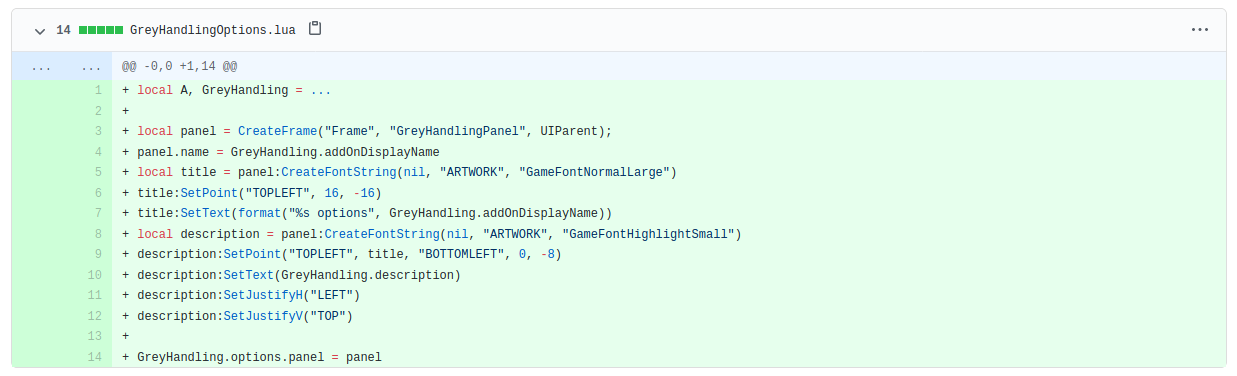
\includegraphics[width=0.8\textwidth]{options_panel_poc.png}
            \source{github.com GreyHandling c01c242dd6a37e2bfeebd6c51a5c7da03fe1b491}
        \end{center}
    \end{block}
}

\frame{\frametitle{Compatibility between WOW retail and WOW classic}
    \begin{block}{Don't overthink it ?}
        \begin{center}
            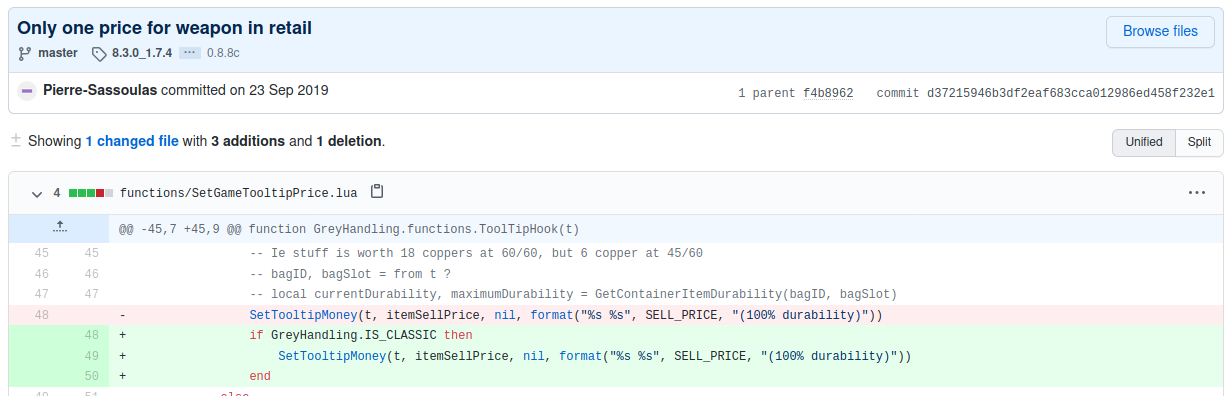
\includegraphics[width=0.8\textwidth]{classic_retail.png}
            \source{github.com GreyHandling d37215946b3df2eaf683cca012986ed458f232e1}
        \end{center}
    \end{block}
    75 \% of users are WOW classic users. So my main branch is for WOW classic,
    and I'm rebasing the WOW retail specific changes on it, but only for major version.
    (1.8.0, but not 1.7.4)
}

\frame{\frametitle{Dependency management}
    \begin{block}{Like javascript in 2005 ?}
        \begin{itemize}
            \item You can't set the version of your dependencies
            \item Any release of another addons can break your addon
            \item A new WOW release by Blizzard will make your addon "deprecated"
            \item You're then supposed to upgrade it, every addon developpers does that at the same time... hope for the best.
        \end{itemize}
    \end{block}

    \begin{block}{What could make this better}
        \begin{itemize}
            \item Dependency management (like pypi, cargo... even npm !)
        \end{itemize}
    \end{block}
}

\frame{\frametitle{Dependency management}
    \begin{block}{What you can do to ease the pain}
        \begin{itemize}
            \item Declare that you're integrated, not integrating, like a boss
            \item Have no dependencies, or integrate them in your code
            \item Use only very big low-level libraries (ACE3, Bitten's SpellFlash)
            \item Accept that your addon will be on fire randomly
        \end{itemize}
    \end{block}
}

\frame{\frametitle{Communication between addons}

    \begin{block}{Communicating between multiple player using your addon}
        \begin{itemize}
            \item Specify your little messaging convention. Keep it short.
            \item I used "v-VersionNumber b-FreeBagSpace" + n * "itemId-itemCount"
            \item Send it via C\_ChatInfo.SendAddonMessage
            \item Listen to "CHAT\_MSG\_ADDON" fired by your own addon
        \end{itemize}
        \begin{center}
            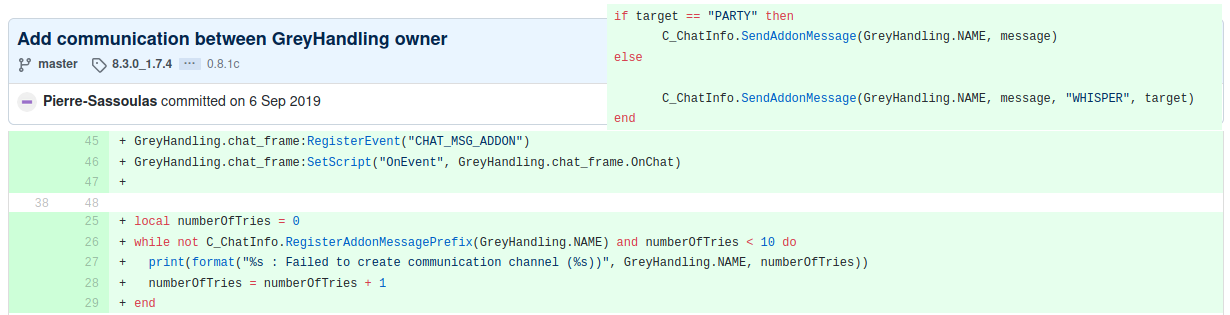
\includegraphics[width=1\textwidth]{communication.png}
            \source{github.com GreyHandling 4e1c9f767ef6c6569ca7e03651a33bf9fe1244b3}
        \end{center}
    \end{block}
}

\frame{\frametitle{Localisation}

    \begin{block}{It's just a dictionary where key are english text}
        \begin{itemize}
            \item WOW gives the localisation
            \item Make english the default if nothing is found
            \item Create a file for each language
            \item Populate the dictionary during init with the right strings
        \end{itemize}
    \end{block}
    \begin{center}
        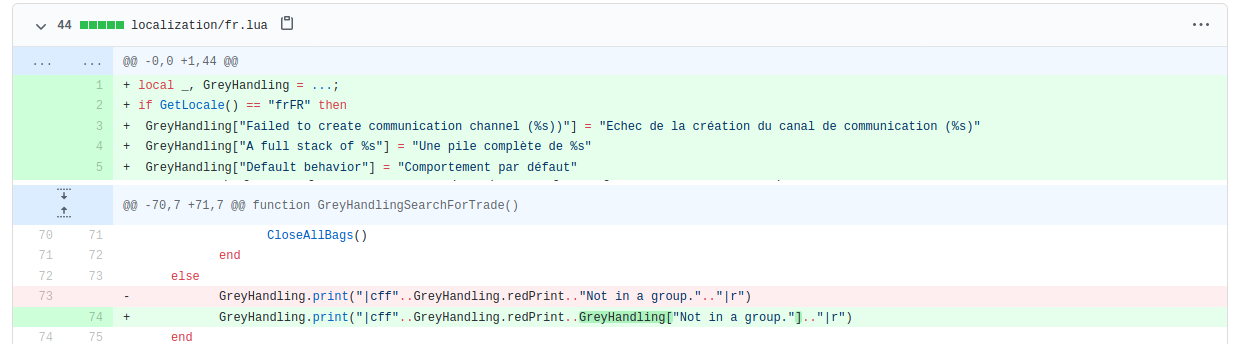
\includegraphics[width=1\textwidth]{l10n.png}
        \source{github.com GreyHandling aa0c366ca9748260ab1b879c57f257b6dfa784a2}
    \end{center}

}

\section{Mainteneer work}

\subsection{Graphic identity}

\frame{\frametitle{Creating a nice icon}

    \begin{block}{Keep the Warcraft's style by reusing existing warcraft icons}
        \begin{itemize}
            \item I think that this is important for visibility in app stores and clean integration in game
            \item You can see all available icons when selecting an icon for a new macro after typing \textbackslash macro
            \item 
\includegraphics[width=0.1\textwidth]{icon/ico1.png}  +
            
\includegraphics[width=0.1\textwidth]{icon/ico2.jpg} +
            NymphAmaryllis's talent =
            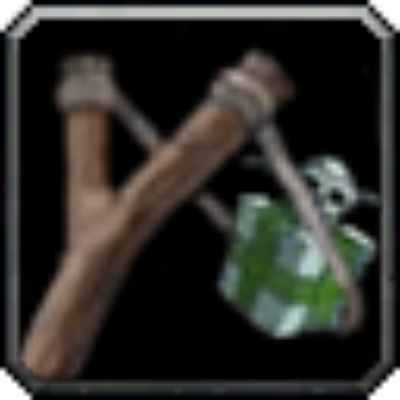
\includegraphics[width=0.1\textwidth]{../art/GreyHandlingTwitchButton.png}
            \item You can also use it in game
        \end{itemize}
        \source{https://www.deviantart.com/nymphamaryllis}
    \end{block}

}

\subsection{Store integration}

\frame{\frametitle{Feedback on Twitch}
    \begin{block}{Not created with issues management in mind}
            \begin{itemize}
            \item But 85 \% of issues will be signaled here
            \item Some user won't go elsewhere whatever you do
            \item So: 
\includegraphics[width=0.65\textwidth]{allow_comment.png}
            \item Deal with it, copy paste the issues elsewhere
        \end{itemize}
    \end{block}
    \begin{center}
        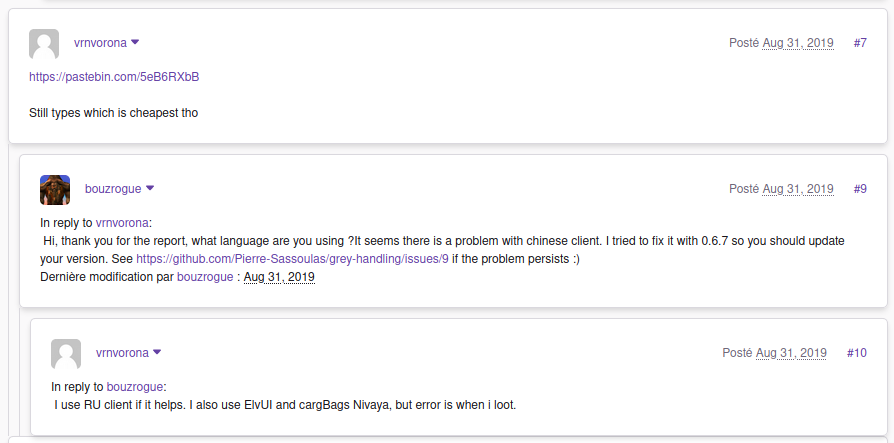
\includegraphics[width=0.65\textwidth]{twitch_issue_report.png}
        \source{curseforge wow/addons/greyhandling}
    \end{center}
}

\frame{\frametitle{Twitch integration}
    \begin{block}{In seven recursive words : Pretty damn convenient}
        \begin{itemize}
            \item Read the documentation (under "Automatic Packaging")
            \item It just works
        \end{itemize}
        \begin{center}
            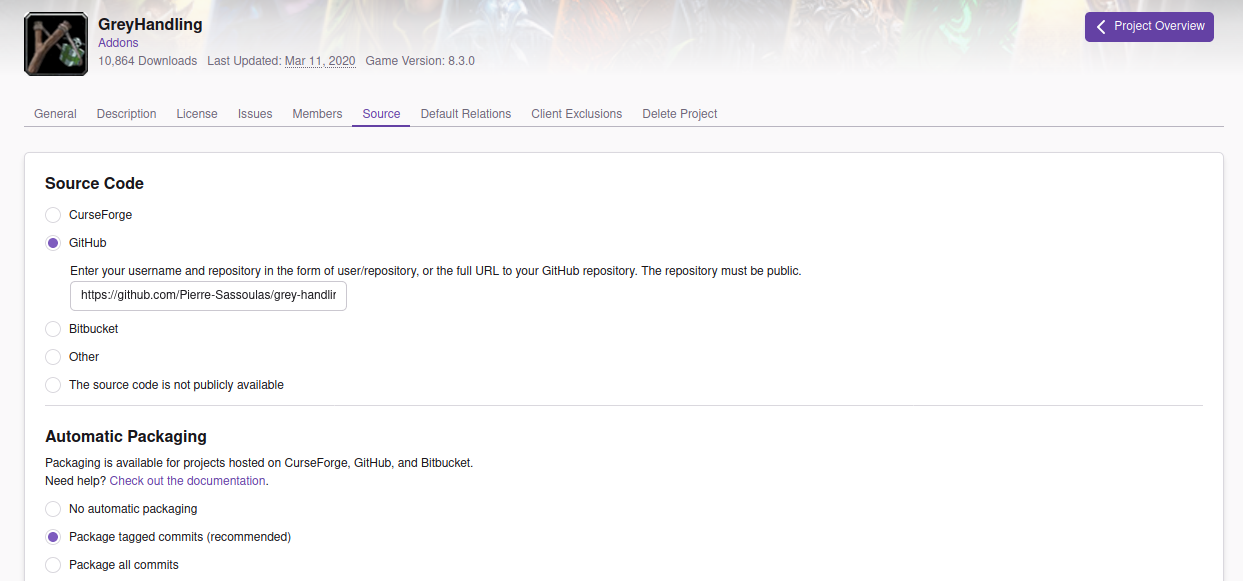
\includegraphics[width=0.85\textwidth]{twitch_integration.png}
            \source{curseforge greyhandling admin panel}
        \end{center}
    \end{block}
}

\frame{\frametitle{WoWInterface integration}

    \begin{block}{Another addon "store": WoWInterface}
        \begin{itemize}
            \item There is no integration with external source repository
            \item So I did not use it and had less users than I could have had
        \end{itemize}
        \begin{center}
            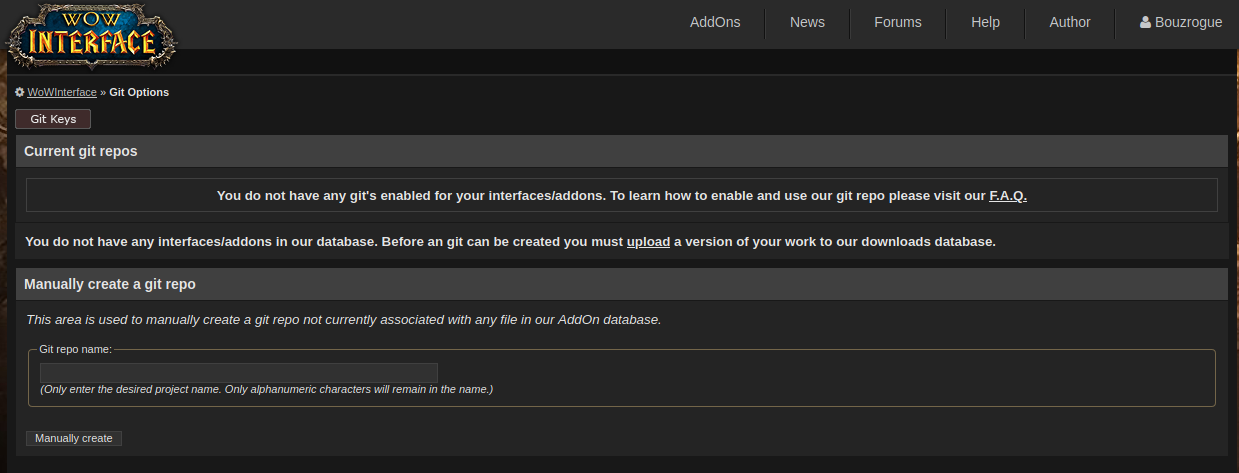
\includegraphics[width=0.85\textwidth]{WoWInterface.png}
            \source{WoWInterface user admin}
        \end{center}
    \end{block}
}

\subsection{Feature requests}

\frame{\frametitle{Feature requests}
    \begin{block}{What was asked by users}
        \begin{itemize}
            \item Being able to change keybinds
            \item Integrate with a lot of bag's addons and trash's addons
            \item Option to be able use half the features
            \item Chinese and Russian language and compatibility
            \item Very quick reports when things break
        \end{itemize}
    \end{block}
}


\frame{\frametitle{Bug fix for russian client}
    \begin{block}{Russian}
        \begin{itemize}
            \item Download the russian client
            \item Create a lua error with the text you need
            \item Add unit test with assertion
        \end{itemize}
    \end{block}

    But maybe you know a russian interested in your addon that can help you ? If not, why are you even bothering ?

    \begin{center}
        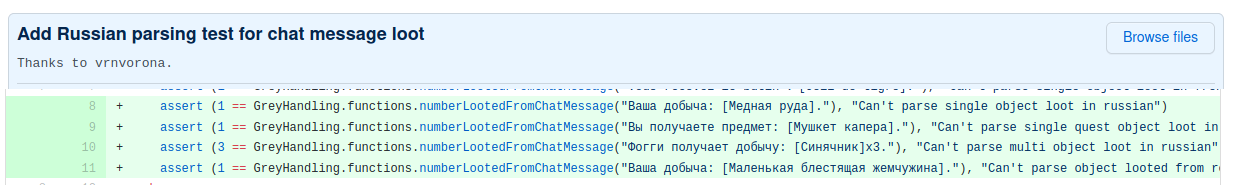
\includegraphics[width=1\textwidth]{russian.png}
        \source{github.com GreyHandling 715953b153aa81045f85225fae9eb394f4936ebd}
    \end{center}
}

\frame{\frametitle{Bug fix for chinese client}

    \begin{block}{Collaborate with a chinese citizen}
        \begin{center}
            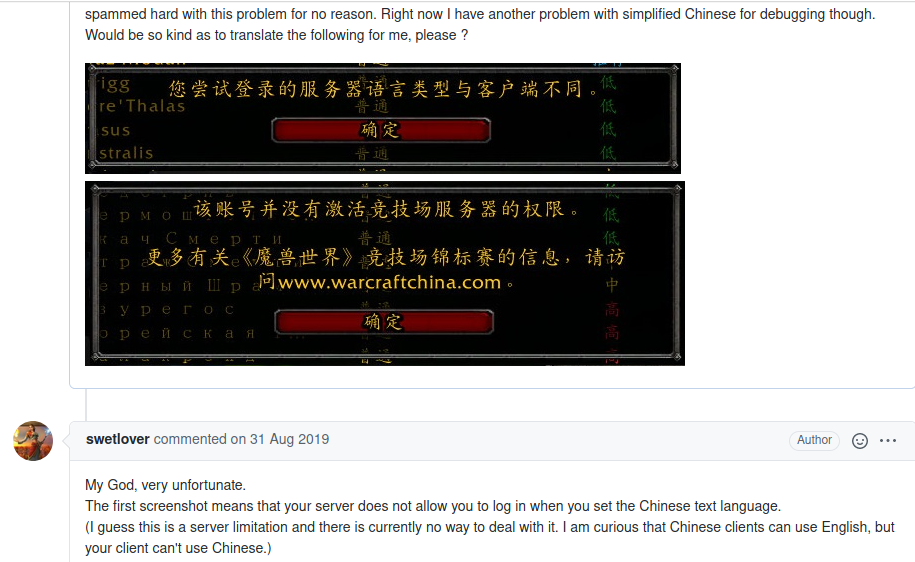
\includegraphics[width=0.7\textwidth]{chinese_discrimination.png}
            \source{github.com GreyHandling issues/9}
        \end{center}
    \end{block}
}


\frame{\frametitle{Asking other mainteneers for help with integration}
    \begin{block}{Do your homework, then don't hesitate}
        \begin{itemize}
            \item Common advices about asking questions apply (See http://www.catb.org/~esr/faqs/smart-questions.html)
            \item TLDR : Show that you at least tried
            \item It's nice to know someone want to integrate your addon so addon developper will probably answer
            \item If they don't it was still worth a try because they can help you A LOT if they do
        \end{itemize}
    \end{block}
}

\frame{\frametitle{ArkInventory integration}
    Thanks to \textbf{arkayenro} for schooling me on event
    programming as well as answering me with copious details really fast.

    \begin{block}{Teach me evenemential programming, sempaï}
        \begin{center}
            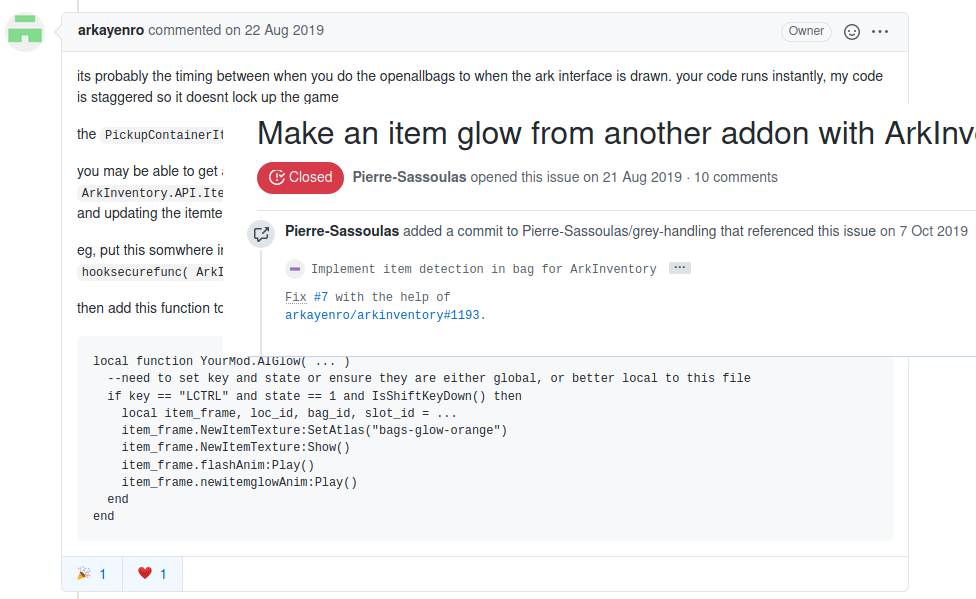
\includegraphics[width=0.7\textwidth]{arkinventory_integration.png}
            \source{github.com, arkayenro/arkinventory issues/1193}
        \end{center}
    \end{block}
}

\frame{\frametitle{ArkInventory integration}
    \begin{center}
        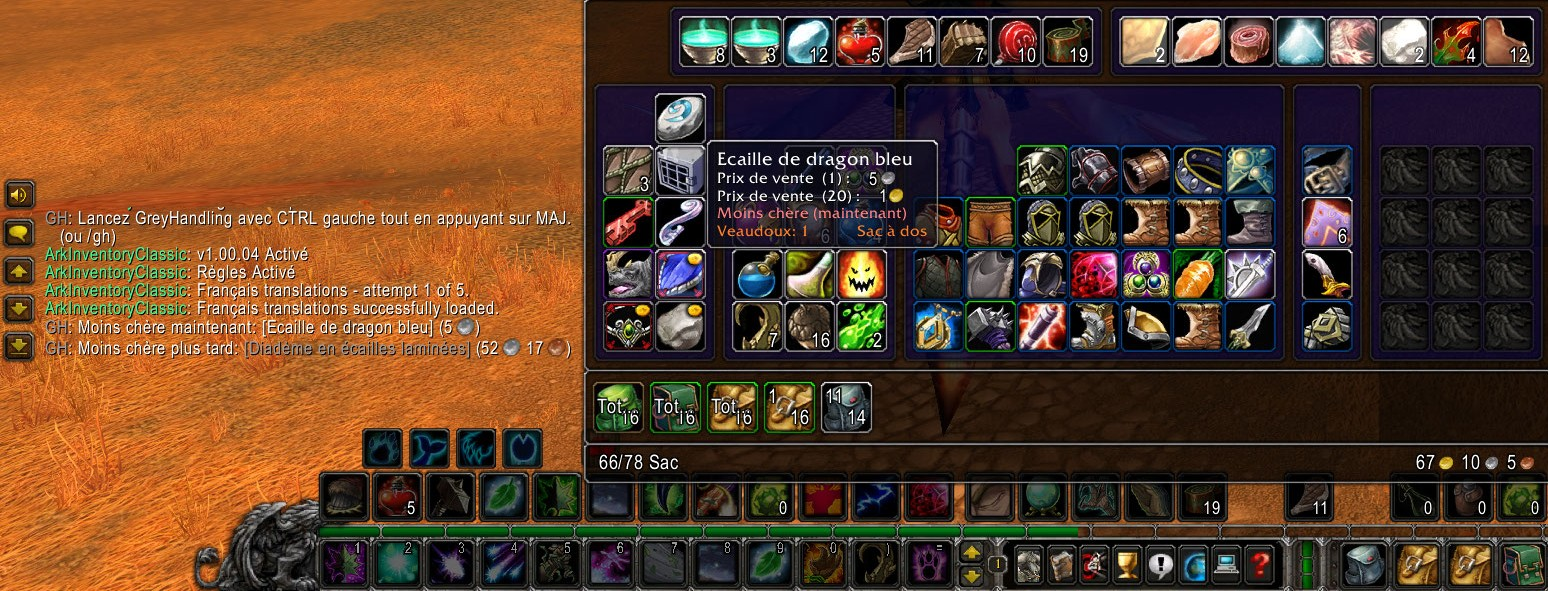
\includegraphics[width=1\textwidth]{arkinventory_result.jpg}
        \source{Bouzrogue, addon developer}
    \end{center}
}

\frame{\frametitle{Bagnon/Combductor integration}
    \begin{block}{Bagnon/Combductor}
        \begin{itemize}
            \item Both addons rely on the \textbf{wildpants} library (https://github.com/tullamods/Wildpants/wiki)
            \item Jaliborc is busy being the maintainer of dozen of major addons, but he does answer questions
        \end{itemize}
        \begin{center}
            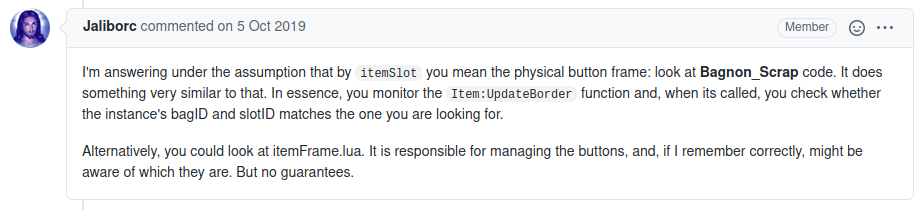
\includegraphics[width=0.9\textwidth]{help_from_jaliborc.png}
            \source{github.com tullamods/Bagnon issues/1007}
        \end{center}
    \end{block}
}

\frame{\frametitle{Demonstration}
\begin{block}{Item throwing with multiple addons in solo play}
    \begin{center}
        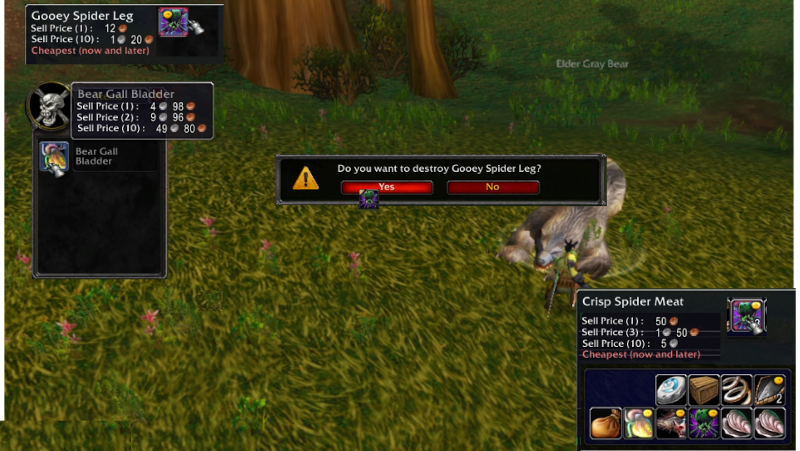
\includegraphics[width=0.7\textwidth]{video_preview.png}
        ~~ \\
        \href{https://youtu.be/soebpWGhydU}{Click this text to view demo}
        \source{Youtube, https://youtu.be/soebpWGhydU}
    \end{center}
\end{block}
}

\frame{\frametitle{Scrap integration}
    \begin{block}{Integrating Scrap}
        \begin{itemize}
            \item Another addon by Jaliborc
            \item The API is clean and easy to use
            \item Permit to create junk list, I needed that
            \item Permit to sell automatically at vendor
            \item 10/10, no problem, great value
        \end{itemize}
        \begin{center}
            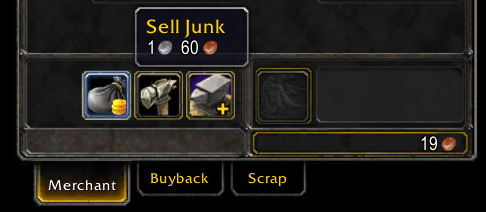
\includegraphics[width=0.4\textwidth]{scrap.png}
            \source{curseforge.com addons/scrap}
        \end{center}
    \end{block}



}

\frame{\frametitle{Peddler integration}
    \begin{block}{Peddler integration}
        \begin{itemize}
            \item Like Scrap but less well known (still used by 50k+ players)
            \item Just had to ask to expose an API
        \end{itemize}
    \end{block}
    \begin{center}
        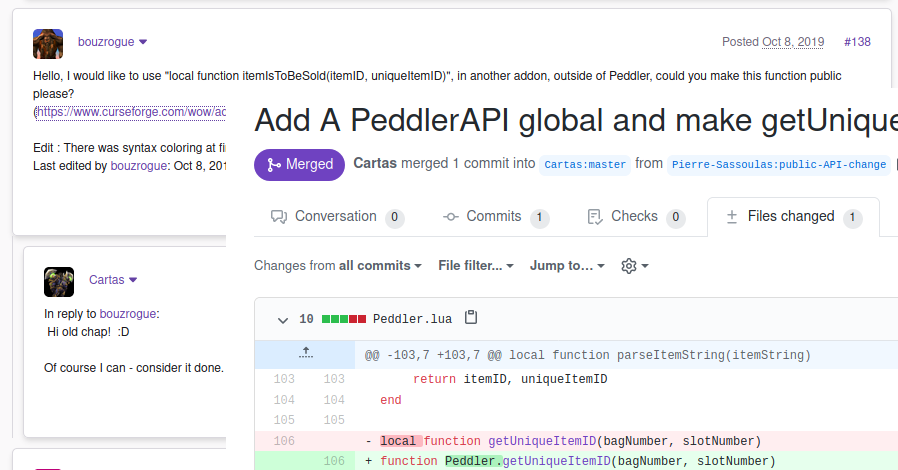
\includegraphics[width=0.7\textwidth]{peddler_integration.png}
        \source{github.com Cartas/Peddler pull/5}
    \end{center}
}

\frame{\frametitle{Scrap and Peddler integration}
    \begin{center}
        An option is dynamically added if Scrap or Peddler is loaded.
        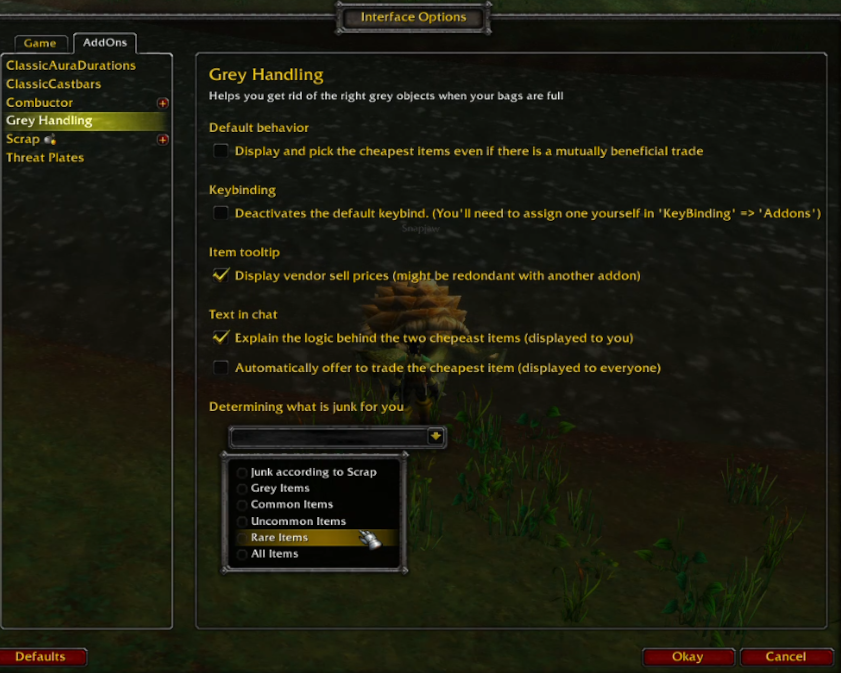
\includegraphics[width=0.65\textwidth]{options_panel_result.png}
        \source{Bouzrogue, addon developer}
    \end{center}
}

\subsection{Bonus}

\frame{\frametitle{Fun algorithmic challenges}

\begin{flushright}
    \begin{quote}
        Much like victims of childhood hardship or abuse can find an escape in fantasy books, victims of
        enterprise programming or freelance web development can find their escape in solving imaginary problems.
    \end{quote}
    \small George Hosu \normalsize
\end{flushright}
    \begin{block}{Bagnon's bag sort is a real problem that you can solve today}
        \begin{itemize}
            \item It's running in parallel
            \item Limiting factor is the number of actual move and number of moved items at the same time
            \item Novel programming problem with no builtin solution
            \item Affect literally millions of persons
        \end{itemize}
    \end{block}

   \source{github.com tullamods/Wildpants pull/48}

}

\frame{\frametitle{Fun algorithmic challenges}
    \begin{block}{Bagnon's bag sorting using a parallelized insertion sort}
        \begin{center}
            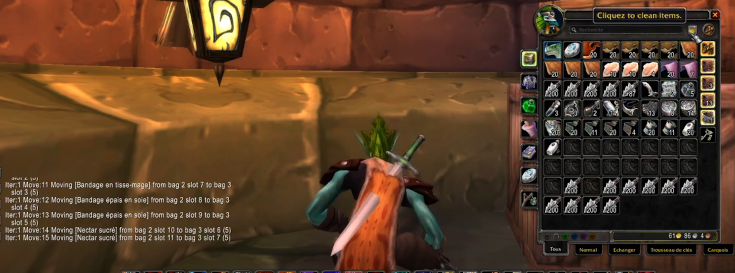
\includegraphics[width=0.9\textwidth]{bagnon_video_preview.png}
            ~~ \\
            \href{https://youtu.be/z1543RQFdaw}{Click this text to view video}
            \source{Youtube, https://youtu.be/z1543RQFdaw}
        \end{center}
    \end{block}
}

\section{Conclusion}

\frame{\frametitle{Conclusion}

    \begin{block}{10/10 - Higly recommend}
        \begin{itemize}
            \item It's not that hard to create an addon without prior knowledge
            \item It's pretty rewarding to have lots of users and feature requests
            \item It gives perspectives on a lot of things
            \item Contributing to other bigger addons permits to impact millions of persons and to  handle interesting algorithmic challenges
        \end{itemize}
    \end{block}

}

\end{document}
